\chapter{Theoretische Grundlagen}
Dieses Kapitel eruiert die theoretischen Grundlagen für die Ausarbeitung, welche für das Verständnis dieser Arbeit notwendig sind und im praktischen Teil angewendet werden.
\section{WordPress als Content-Management-System}
WordPress ist ein freies, unter der \gls{gnu} \gls{gpl} v2 lizenziertes Content-Management-System und mit einem Marktanteil von 61,1\% das weltweit am häufigsten verwendete CMS. \cite{statista2025cms}
Die Plattform zeichnet sich durch seine flexibilität, erweiterbarkeit und bedienbarkeit aus, was Wordpress zu einer Lösung für simple Webseiten und Blogs bis hin zu komplexe Web-Applikationen macht. \cite{patel2019review}
Die technische Struktur verfolgt ein modulares Paradigma, das eine klare Trennung zwischen Kernfunktionen, Design und Erweiterungen ermöglicht:
\begin{itemize}

 \item Themes: Kontrollieren die Präsentationslogik und das Design der Webseite

 \item Plugins: Erweitern die Funktionalität

 \item Core System: Stellt die grundlegenden Funktionen des CMS bereit

\end{itemize}
Technisch gesehen besteht Wordpress aus einer \gls{php}-basierten Architektur in Verbindung mit der persistenten Speicherlösung \gls{mysql} als relationale Datenbank.
Durch diese weit verbreiteten Technologien ist WordPress mit den meisten gängigen Hosting-Umgebungen kompatibel.
Grundlage hierfür ist ein Webserver, welcher PHP und MySQL unterstützt.
Offiziell ist Apache oder Nginx empfohlen \cite{wordpress2024requirements}.

Darüber hinaus bietet Wordpress eine \gls{rest}-\gls{api} mit der eine entkoppelte Inhaltsverwaltung möglich ist und Inhalte über das \gls{http}-Protokoll in verschiedene Anwendungen und Plattformen integriert werden können.
\newpage
\textbf{WordPress Coding Standards und Code-Qualität}\\
Wordpress Coding Standards dienen als Richtlinien und Best Practises für Entwickler die an Wordpress Projekten arbeiten.
Diese Standards haben sich in der Wordpress Community etabliert und ermöglichen eine konsistente Codestruktur.
Hintergrund ist es die Codebasis für bessere Wartbarkeit und kollaborative Arbeit zu strukturieren.
Für die Ausarbeitung der Weiterentwicklung von Charigame sollen die offiziellen Wordpress Coding Standards beachtet und umgesetzt werden.


\section{Plugin-Entwicklung mit WordPress}

Die offizielle WordPress-Definition besagt: \glqq Plugins sind Codepakete, die die Kernfunktionalität von WordPress erweitern.
WordPress-Plugins bestehen aus PHP-Code und können weitere Assets wie Bilder,
CSS und JavaScript enthalten\grqq{} \cite{wordpress2024plugin} (eigene Übersetzung).
\\
Für die Entwicklung solcher Plugins ist grundlegend ein tiefergehendes Verständnis des Wordpress-CMS vorausgesetzt.
Die Grundlagen sowie weiterführende Themengebiete sollen im Folgenden ermittelt werden.



\subsection{Grundlagen der Plugin-Architektur}

Die Entwicklung von Plugins in WordPress setzt ein Basiswissen der Dateistruktur und des internen Aufbaus des Content-Management-Systems voraus.
Insbesondere ist es erforderlich, die Plugin-bezogenen Dateien korrekt zu strukturieren und im entsprechenden Verzeichnis innerhalb der WordPress-Installation zu platzieren.\\\\
Plugins werden standardmäßig im Verzeichnis \texttt{wp-content/plugins} abgelegt.
Jeder Plugin-Ordner enthält dabei alle notwendigen Dateien zur Funktionalität des jeweiligen Moduls.\\\\
Im folgenden Schaubild ist eine typische, nicht modifizierte Verzeichnisstruktur einer WordPress-Installation dargestellt.
Diese dient als Ausgangspunkt für die Entwicklung und Integration von Plugins:

\begin{figure}[tbh]
 \centering
 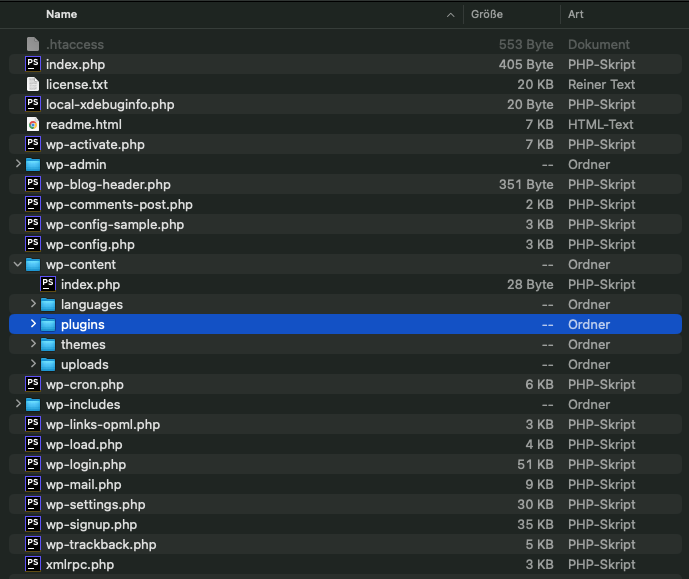
\includegraphics[width=0.88\textwidth]{wordpress_ordner_aufbau}
 \caption{Unveränderte WordPress-Verzeichnisstruktur (6.8.2)}
 \label{fig:wordpress-verzeichnis}
\end{figure}
\newpage
Abbildung 2.1 visualisiert, dass sich im wp-content Ordner bereits initial in der Standardkonfiguration von Wordpress das Verzeichnis \texttt{plugins} befindet.
Der \texttt{plugins} Ordner ist die zentrale Destination für alle im Wordpress System erstellten Erweiterungen.
Die nachfolgende Untersuchung berücksichtigt weitere Bestandteile von WordPress-Plugins, die fortlaufend detailliert beschrieben werden.
\\\\\\
\textbf{Aufbau, Plugin-Header und Metadateien}

Für die Entwicklung von WordPress-Plugins empfehlen die offiziellen WordPress Developer Resources eine klare und strukturierte Ordnerorganisation\cite{wordpress2024BestPractices}.
Als Empfohlen wird folgende grundlegende Verzeichnisstruktur vorgeschlagen:
\\\\\\
\begin{lstlisting}[caption={Beispielhafte Plugin-Verzeichnisstruktur in WordPress}, label={lst:plugin-structure}]
/plugin-name
│
├── plugin-name.php
├── uninstall.php
│
├── /languages
├── /includes
│
├── /admin
│   ├── /js
│   ├── /css
│   └── /images
│
└── /public
    ├── /js
    ├── /css
    └── /images
\end{lstlisting}

Die plugin-name.php gibt im oben gezeigten Beispielaufbau die zentrale Plugindatei an.
Diese Datei muss damit der Ordner als Plugin verstanden wird einen von Wordpress vorgegebene Headerstrutkur enthalten.
Das Minimum des Header ist wie folgt definiert:

\begin{lstlisting}[caption={Minimaler Plugin-Header in WordPress}, label={lst:plugin-header}]
<?php
/*
 * Plugin Name: YOUR PLUGIN NAME
 */
\end{lstlisting}

Darüber hinaus können weitere optionale Felder definiert werden wie:
\texttt{Author URI} für die Website des Plugin-Entwicklers, \texttt{Text Domain}
zur Internationalisierung und \texttt{Domain Path} für den Pfad zu Sprachdateien.
Alle möglichen Felder werden in der folgenden Tabelle aufgeführt:
\renewcommand{\arraystretch}{1.3}

\begin{longtable}{>{\bfseries}p{4cm} p{10cm}}
 \caption{Übersicht der Plugin-Header-Felder in WordPress} \\
 \hline
 Feldname & Beschreibung \\
 \hline
 \endfirsthead

 \multicolumn{2}{l}{\textit{Fortsetzung von vorheriger Seite}} \\
 \hline
 Feldname & Beschreibung \\
 \hline
 \endhead

 \hline
 \multicolumn{2}{r}{\textit{Fortsetzung auf nächster Seite}} \\
 \endfoot

 \hline
 \endlastfoot

 Plugin Name (erforderlich) & Der Name des Plugins, wie er in der Plugin-Übersicht im WordPress-Adminbereich angezeigt wird. \\
 Plugin URI & Eine eindeutige URL zur Startseite des Plugins, idealerweise auf der eigenen Website. WordPress.org-URLs sind hier nicht erlaubt. \\
 Description & Eine kurze Beschreibung des Plugins (max. 140 Zeichen), wie sie im WordPress-Adminbereich angezeigt wird. \\
 Version & Die aktuelle Versionsnummer des Plugins, z.\,B. \texttt{1.0} oder \texttt{1.0.3}. \\
 Requires at least & Die minimale WordPress-Version, mit der das Plugin kompatibel ist. \\
 Requires PHP & Die minimale benötigte PHP-Version für das Plugin. \\
 Author & Der Name des Autors oder der Autoren des Plugins. Mehrere Autoren können durch Kommas getrennt angegeben werden. \\
 Author URI & Die Website des Autors oder ein öffentliches Profil, z.\,B. auf WordPress.org. \\
 License & Die Kurzbezeichnung der Lizenz, unter der das Plugin veröffentlicht wird (z.\,B. \texttt{GPLv2}). \\
 License URI & Ein Link zum vollständigen Lizenztext (z.\,B. \url{https://www.gnu.org/licenses/gpl-2.0.html}). \\
 Text Domain & Die Textdomain für die Internationalisierung des Plugins, erforderlich für Übersetzungen mit \texttt{gettext}. \\
 Domain Path & Das Verzeichnis, in dem WordPress die Übersetzungsdateien findet (z.\,B. \texttt{/languages}). \\
 Network & Gibt an, ob das Plugin netzwerkweit (Multisite) aktiviert werden kann. Nur \texttt{true} ist erlaubt, andernfalls Feld weglassen. \\
 Update URI & Eine eindeutige URI zur Updatequelle, um versehentliche Überschreibungen durch gleichnamige Plugins im WordPress.org-Verzeichnis zu vermeiden. \\
 Requires Plugins & Eine durch Kommas getrennte Liste von Plugin-Slugs aus dem WordPress.org-Verzeichnis, die als Abhängigkeit benötigt werden. Kommas innerhalb der Slugs sind nicht erlaubt. \\
\end{longtable}

\newpage
\textbf{Hooks: Action und Filter}\\\\
Es gibt eine Kardinalregel in der Wordpress Entwicklung die besagt: Don’t touch WordPress core. %TODO: https://developer.wordpress.org/plugins/intro/ maybe verlinken?
Damit Anpassungen an bestehende Funktionalitäten möglich sind gibt es Hooks und Filter.
Hooks erlauben es an spezifischen Stellen einzugreifen, um das Verhalten von Wordpress zu ändern ohne dabei die Kern-Dateien bearbeiten zu müssen.
Allgemein gibt es zwei Arten von hooks in Wordpress: Actions und Filter.
Mit Actions können Funktionen hinzugefügt oder geändert werden.
Filter wiederum ändern Inhalte, während diese geladen und dem Website-Nutzer angezeigt werden.
Hooks sind nicht nur für die Plugin-Entwicklung gedacht, sondern werden ebenfalls häufig verwendet, um Standardfunktionen durch den Wordpress-Kern selbst bereitzustellen.

Drei sehr wichtige Hooks im Bereich der Plugins zählen der \texttt{register\_activation\_hook()}, \texttt{register\_deactivation\_hook()} und der \texttt{register\_uninstall\_hook()}.

\begin{itemize}
 \item register\_activation\_hook(): Dieser Hook wird ausgeführt, wenn das Plugin im Wordpress-Backend aktiviert wird. Dies wird oftmals verwendet um Funktionen zwecks Einrichtung des Plugins bereitzustellen.
 \item register\_deactivation\_hook(): Der Deaktivierung-Hook wird ausgeführt, wenn das Plugin deaktiviert wird. Diese Funktion ermöglicht es die vom Plugin temporär gespeicherten Daten und Einträge zu entfernen.
 \item register\_uninstall\_hook(): Die Ausführung hier findet statt, wenn das Plugin aus dem Backend gelöscht wird. Die Verwendung zielt häufig darauf ab alle vom Plugin erstellen Optionen oder Datenbanktabellen restlos zu löschen.
\end{itemize}

%Plugin-Struktur und -Organisation

%Das WordPress Hook-System verstehen

%Plugin-Header und Metadaten

%Aktivierung und Deaktivierung von Plugins

%Plugin-Hauptdatei und Ordnerstruktur

\subsection{Best Practises in der Plugin-Programmierung}\
Die Wordpress Developer Resources geben dem Entwickler einige Best Practises vor, welche helfen den Code zu organisieren.
Ferner wird durch die Hinweise sichergestellt, dass der Code gut mit dem Wordpress Kern und anderen Plugins funktioniert.
Nachfolgend sollen wichtige Best Practise aufgeführt werden, welche im Verlauf der Arbeit mit in der Konzeption berücksichtigt werden.
\\
\\
\textbf{Vermeiden von Namenskonflikten}\\\\
Namenskollisionen können durch die gleiche Benennung von Variablen, Funktionen oder Klassen zustandekommen.
Um einen solchen Namenskonflikt zu vermeiden ist es empfohlen einen globalen Namenspace zu definieren.
Dieser Namespace ermöglicht das überschreiben von anderen Variablen, Funktionen und Plugins.
Variablen die innerhalb von Funktionen oder Klassen definiert sind, sind hiervon nicht betroffen.
\\
\\
\\
\textbf{Voranstellen eines Prefix}\\\\
Unter Zuhilfenahme eines Prefix können potenzielle Konflikte im Hinblick auf Aufrufe und Ausführungen mit anderen Plugins verhindert werden.
Das Handbuch empfiehlt hierzu ein einzigartiges Wort, welches vor verschiedene deklarationen vorangestellt wird.
Auf das Projekt ChariGame gemünzte Projekt könnte dies dann wie folgt aussehen:
\begin{itemize}
 \item function charigame\_save\_post();
 \item define ('CHARIGAME\_LICENSE', true);
 \item class CHARIGAME\_Admin{}
 \item namespace ChariGame;
 \item update\_option('charigame\_settings', \$settings)
\end{itemize}
\vspace{1em}
\textbf{Prüfung vorhandener Implementierungen}\\\\
Damit der Code Robust  und weniger fehleranfällig ist, gilt es auf bestehende Implementationen zu prüfen.
Dies geschieht unter Zuhilfenahme der folgenden von PHP zur Verfügung gestellten Funktionen:
\begin{itemize}
 \item Variablen: isset()
 \item Function\_exists() %NICHT BENÖTIGT IN EIGENEM NAMESPACE
 \item Classes class\_exists()
 \item Constants defined()
\end{itemize}
\vspace{1em}
\textbf{Architekturmuster}\\\\
Die Wordpress Developer Resources geben eine Hand voll mögliche Architekturmuster vor.
Diese können grob in drei Variationen kategorisiert werden:
\begin{itemize}
 \item Einzelne Plugin-Datei, die Funktionen enthält
 \item Einzelne Plugin-Datei, die eine Klasse, ein instanziiertes Objekt und optional Funktionen enthält
 \item Haupt-Plugin-Datei, dann eine oder mehrere Klassendateien
\end{itemize}

Je nachdem welchen Umfang das Plugin anstrebt, gilt es die passende Lösung des Architekturmusters zu wählen.
Ein einzelne Plugin-Datei, die Funktionen enthält stellt eine solide Basis für ein kleines Plugin zur Verfügung.
Die Variante eine Haupt-Plugin-Datei zu erstellen und mehrere Klassendateien aufzubauen bietet sich eher für Plugins mit einer größeren Codebasis an.

\subsection{Plugin Security und Privacy}
Ein wichtiger Aspekt bei der Programmierung von Wordpress Plugins ist die Plugin Security und Privacy.
Damit die Sicherheit von Eingaben gegeben ist, werden Methoden wie Validating, Sanatizing und Escaping genutzt.

\textbf{Validating}

\begin{quote}
 Das Validierung von Eingaben ist der Prozess, bei dem Daten anhand eines vordefinierten Musters (oder mehrerer Muster) mit einem eindeutigen Ergebnis getestet werden: gültig oder ungültig.
 Die Validierung ist im Vergleich zur Bereinigung ein spezifischerer Ansatz, aber beide haben ihre Berechtigung.
 \\[0.5em]
 \emph{(eigene Übersetzung nach \cite{wordpress2024plugin_validation})}
\end{quote}

Es werden auch seitens der Wordpress Developer Ressourcen einfache Validierungsbeispiele genannt:
\begin{itemize}
\item Überprüfung, ob Pflichtfelder ausgefüllt wurden
\item Überprüfung, ob eine eingegebene Telefonnummer nur Zahlen und Satzzeichen enthält
\item Überprüfung, ob eine eingegebene Zeichenfolge eine von fünf gültigen Optionen ist
\item Überprüfung, ob ein Mengenfeld größer als 0 ist
\end{itemize}
Die Validierung selbst wird in verschiedene Philosophien gegliedert, die nun kurz exemplarisch aufgefasst werden:
\begin{table}[h]
 \centering
 \renewcommand{\arraystretch}{1.3}
 \begin{tabular}{|p{3cm}|p{5cm}|p{6cm}|}
  \hline
  \textbf{Philosophie} & \textbf{Beschreibung} & \textbf{Beispiel Anwendung} \\
  \hline
  Safelist \newline (Allowlist)
  & Nur Werte aus einer vordefinierten Liste erlauben. Alles andere wird abgelehnt.
  & Dropdown-Auswahl für Sortieroptionen (z.\,B. ``date``, ``author``). Nur erlaubte Keys werden akzeptiert. \\
  \hline
  Blocklist \newline (Denylist)
  & Bestimmte bekannte, unerwünschte Werte verbieten. Unsicher, da neue unerlaubte Werte nicht erfasst werden.
  & Sperren von bekannten schädlichen Dateiendungen (z.\,B. ``.exe``, ``.bat``). \\
  \hline
  Format Detection
  & Prüfen, ob Eingabe einem bestimmten Muster entspricht.
  & Postleitzahl-Validierung mit Regex, E-Mail-Prüfung mit \texttt{is\_email()}, nur Ziffern mit \texttt{ctype\_digit()}. \\
  \hline
  Format Correction (Sanitization)
  & Eingaben akzeptieren, aber in ein sicheres Format umwandeln.
  & Benutzername \newline mit \texttt{sanitize\_title()}, Typ-Cast von String zu Integer \texttt{(int)\$input}. \\
  \hline
 \end{tabular}
 \caption{Übersicht Validierungs-Philosophien mit Beispielen}
\end{table}

\newpage
Wenn keine Validierung möglich ist bedienen sich Wordpress Entwickler der Möglichkeit des Sanatizing und Escaping von Werten.

\textbf{Sanitizing}
\begin{quote}
 Die Bereinigung von Eingaben ist der Prozess der Sicherung/Bereinigung/Filterung von Eingabedaten.
 Die Validierung ist der Bereinigung vorzuziehen, da sie spezifischer ist.
 Wenn jedoch eine „spezifischere“ Lösung nicht möglich ist, ist die Bereinigung die nächstbeste Option.
 \\[0.5em]
 \emph{(eigene Übersetzung nach \cite{wordpress2024plugin_sanitizing})}
\end{quote}


Bevor also Daten, die von Nutzenden stammen, in der Datenbank abgelegt oder weiterverarbeitet werden,
sollten sie bereinigt werden, um sowohl Sicherheitslücken als auch ungewollte Inhalte zu vermeiden.
Dafür stellt WordPress verschiedene Funktionen bereit, die sicherstellen, dass Eingaben ausschließlich
die vorgesehenen Zeichen oder Strukturen enthalten.
Ein häufig genutztes Beispiel ist die Verwendung von \texttt{sanitize\_text\_field()} für Freitextfelder.
Nachfolgend werden die seitens Wordpress bereitgestellten Funktionen erläutert:

\begin{table}[h]
 \centering
 \begin{tabular}{|l|p{8cm}|}
  \hline
  \textbf{Funktion} & \textbf{Beschreibung} \\
  \hline
  \texttt{sanitize\_text\_field()} & Entfernt Tags, ungültige UTF-8-Zeichen, Zeilenumbrüche, Tabs und überflüssige Leerzeichen. \\
  \hline
  \texttt{sanitize\_email()} & Validiert und bereinigt eine E-Mail-Adresse. \\
  \hline
  \texttt{sanitize\_file\_name()} & Entfernt unerlaubte Zeichen aus Dateinamen. \\
  \hline
  \texttt{sanitize\_hex\_color()} & Prüft und bereinigt Hex-Farbwerte (\#RRGGBB). \\
  \hline
  \texttt{sanitize\_html\_class()} & Bereinigt Klassennamen für HTML-Attribute. \\
  \hline
  \texttt{sanitize\_key()} & Bereinigt Array-Keys oder Optionsnamen. \\
  \hline
  \texttt{sanitize\_option()} & Bereinigt Optionswerte in der Datenbank. \\
  \hline
  \texttt{sanitize\_title()} & Macht einen String zu einem URL-freundlichen Titel. \\
  \hline
  \texttt{sanitize\_user()} & Bereinigt Benutzernamen. \\
  \hline
  \texttt{wp\_kses()} & Filtert HTML nach erlaubten Tags/Attributen. \\
  \hline
  \texttt{wp\_kses\_post()} & Wie \texttt{wp\_kses()}, aber mit Standardregeln für Posts. \\
  \hline
 \end{tabular}
 \caption{Auswahl wichtiger WordPress-Sanitization-Funktionen}
\end{table}

\newpage

\textbf{Escaping}\\\\
Escaping transformiert Ausgabedaten so, dass gefährliche Zeichen (z.\,B. `<` wird zu `\&lt;`) nicht mehr als Code interpretiert werden. Dies verhindert XSS-Angriffe.\\\\
Das Prinzip lautet: Daten unverändert speichern, erst bei der Ausgabe escapieren. WordPress bietet kontextspezifische Funktionen wie \texttt{esc\_html()}, \texttt{esc\_attr()}, \texttt{esc\_url()} und \texttt{esc\_js()}.
Die richtige Funktionswahl je nach Ausgabekontext ist entscheidend für die Sicherheit.
Genau wie beim Sanatizing bietet Wordpress hier ein Set an Funktionen, welche speziell für das Escaping genutzt werden.

\begin{table}[h]
 \centering
 \begin{tabular}{|l|p{9cm}|}
  \hline
  \textbf{Funktion} & \textbf{Anwendungsfall / Beschreibung} \\
  \hline
  \texttt{esc\_html()} & Escaped Text für den Einsatz innerhalb von HTML-Elementen. Entfernt sämtliches HTML. \\
  \hline
  \texttt{esc\_attr()} & Für Werte innerhalb von HTML-Attributen, z.\,B. \texttt{<input value="...">}. \\
  \hline
  \texttt{esc\_url()} & Für URLs in \texttt{src} oder \texttt{href}-Attributen. \\
  \hline
  \texttt{esc\_url\_raw()} & Roh-URL-Escaping für Speicherung in der Datenbank oder nicht-encodierte Weitergabe. \\
  \hline
  \texttt{esc\_js()} & Für Inline-JavaScript oder Übergabe von Variablen in Skripte. \\
  \hline
  \texttt{esc\_xml()} & Absicherung von Ausgaben in XML-/XSL-Kontexten. \\
  \hline
  \texttt{esc\_textarea()} & Encodiert Texte für die Verwendung innerhalb eines \texttt{<textarea>} Elements. \\
  \hline
  \texttt{wp\_kses()} & Filtert HTML-Inhalte und erlaubt nur eine definierte Menge an Tags/Attributen. \\
  \hline
  \texttt{wp\_kses\_post()} & Variante von \texttt{wp\_kses()}, die die Standardmenge an Post-HTML erlaubt. \\
  \hline
  \texttt{wp\_kses\_data()} & Variante von \texttt{wp\_kses()}, die nur HTML erlaubt, das in Kommentaren zugelassen ist. \\
  \hline
 \end{tabular}
 \caption{Überblick zentraler Escaping-Funktionen in WordPress}
 \label{tab:escaping}
\end{table}

Ein wichtiger Grundsatz ist das \emph{späte Escaping}: Daten sollten erst unmittelbar vor der Ausgabe escaped werden.
Dadurch wird die Code-Überprüfung vereinfacht, das Fehlerrisiko verringert und die Anwendung widerstandsfähiger gegen zukünftige Anpassungen.
Wenn ein spätes Escaping nicht umsetzbar ist (etwa bei generiertem JavaScript-Code), muss der Entwickler sicherstellen, dass Variablen bereits in einer als \enquote{sicher} gekennzeichneten Form vorliegen (z.\,B. \texttt{\$variable\_escaped}).

\textbf{Nonces}

Ein Nonce (number used once) ist ein Sicherheitsmechanismus in WordPress zum Schutz von URLs und Formularen vor unbefugten Manipulationen.
Insbesondere wird der Schutz vor Cross-Site Request Forgery (CSRF) sichergestellt.
Anders als die Definition handelt es sich nicht um Einmalzahlen, sondern um Hash-Werte.
Diese Hashwerte sind für einen bestimmten Benutzer und Kontext über eine begrenzte Zeit gültig (Standard: 12–24 Stunden).

Erstellung: \texttt{wp\_create\_nonce('action')}, \texttt{wp\_nonce\_url()}, \texttt{wp\_nonce\_field()}

Validierung: \texttt{wp\_verify\_nonce()}, \texttt{check\_admin\_referer()}, \texttt{check\_ajax\_referer()}

Sie sollten stets aktionsspezifisch sein und niemals als alleinige Sicherheitsmaßnahme dienen.





\subsection{Weiterführende Funktionen und Paradigma}
In diesem Kapitel sind weitere für da Projekt verwendete Funktionen und Paradigmen aus Wordpress aufgeführt.


Hier noch überlegen welche Funktionen und Paradigmen aufgeführt werden sollten. Effektiv bisschen filler für das kommende dann?
Meta-Daten // Meta Boxes für Post-Bearbeitung

Einstellungsseiten mit Settings \gls{api}

Integration mit \gls{acf} für erweiterte Felder

Shortcodes entwickeln und registrieren

\gls{css} und JavaScript richtig einbinden

Gutenberg Block-Entwicklung (optional)

Custom \gls{rest} \gls{api} Endpoints erstellen

Daten über \gls{http}-Requests bereitstellen

Authentifizierung und Berechtigungen

AJAX-Funktionalität implementieren

Admin-Menüs und Unterseiten erstellen

WordPress Database \gls{api} für Datenbankoperationen

Custom Post Types und Custom Fields

Settings und Options verwalten

Caching mit Transients

Plugin für WordPress Repository vorbereiten

Versionskontrolle und Updates

Lizenzierung unter \gls{gpl}

Plugin-Testing und Qualitätssicherung

Cron

\section{Gutenberg-Editor: Konzept und technische Grundlagen}
\begin{quote}
    Der Block-Editor ist ein modernes Paradigma für die Erstellung und Veröffentlichung von WordPress-Websites.
    Er verwendet ein modulares System aus Blöcken zum Erstellen und Formatieren von Inhalten und wurde entwickelt,
    um reichhaltige und flexible Layouts für Websites und digitale Produkte zu erstellen.
    \\[0.5em]
    \emph{(eigene Übersetzung nach \cite{wordpress2024plugin_blockeditor})}
\end{quote}



Ein Block ist ein eigenständiges Element wie beispielsweise ein Absatz, eine Überschrift, ein Medienelement oder eine Einbettung.
Jeder Block wird als separates Element mit individuellen Bearbeitungs- und Formatierungsoptionen behandelt.
Wenn alle diese Komponenten zusammengefügt werden, bilden sie den Inhalt der Seite oder des Beitrags, der dann in der WordPress-Datenbank gespeichert wird.
\\\\
Die Developer Resources geben Entwicklern Grundlagen der Blockentwicklung mit, welche nachfolgend erläutert werden.

\subsection{Dateistruktur eines Blocks}

Wenn ein Block entwickelt wird, ist es empfohlen diesen als Plugin und nicht innerhalb des Themes zu registrieren.
Diese Methode wird empfohlen, damit der erstellte Block unabhängig vom verwendeten Theme genutzt werden kann.

%TODO: HIER BILD ERSTELLEN STRUKTUR EINES BLOCKS



Die Relevanz des Editors wird durch die Erhobene Statistik der Seite Gutenberg in Numbers deutlich.
Demnach beträgt die Anzahl aktiver Installationen des Gutenberg-Editors auf WordPress- und Jetpack-Seiten aktuell 87,3 Mio.
Innerhalb der letzten drei Jahre wurden 282 Mio. Beiträge mit dem Gutenberg-Editor erstellt.
Die Daten basieren auf einem Dreijahreszeitraum und umfassen nur WordPress.com- und Jetpack-Seiten, die die Nutzung des Editors melden.

This section provides an introduction to the most relevant concepts in block development. Use the following links to learn more:

File structure of a block: The purpose of each file that composes a block plugin, the relationships between them, and their role in the block output.
block.json: How a block is defined using its block.json metadata and some relevant properties of this file (such as attributes and supports).
Registration of a block: How a block is registered on both the server and in the client.
Block wrapper: How to apply the proper attributes to the block’s markup wrapper.
The block in the Editor: How a block, as a React component, is loaded in the Block Editor and an overview of its structure.
Markup representation of a block: How blocks are represented in the database, theme templates, and patterns.
Static or Dynamic rendering of a block: How blocks generate their front-end output either dynamically or statically.
JavaScript in the Block Editor: How to work with modern JavaScript when developing for the Block Editor.


\section{Gamification im Kontext digitaler Anwendungen}
https://www.bpb.de/themen/kultur/digitale-spiele/504558/gamification-grundbegriffe-chancen-und-risiken/
https://www.bidt.digital/phaenomene/gamification-und-digitale-partizipation-neue-impulse-fuer-die-demokratie/
https://reposit.haw-hamburg.de/bitstream/20.500.12738/7511/1/BA_Ibel.pdf

\section{Überblick über Coperate Responsibility und Charity-Plattformen}

Marktanalyse für Charigame
Marktumfeld und Trends
Gamification-Markt in Deutschland
Der Gamification-Markt in Deutschland zeigt eine positive Entwicklung mit signifikantem Wachstum. Unternehmen aus verschiedenen Branchen wie Gesundheitswesen, Finanzdienstleistungen und E-Learning setzen zunehmend auf gamifizierte Lösungen, um die Kundeninteraktion und Mitarbeiterbindung zu verbessern.

Europa verzeichnet insgesamt ein starkes Wachstum, das durch Unternehmensinvestitionen in Gamification-Konferenzen und KI-gestützte Engagement-Lösungen angetrieben wird. Länder wie Deutschland, Großbritannien und Frankreich sind Vorreiter bei der Gamification in Einzelhandel, HR und Gesundheitswesen.

CSR-Trends 2025
Aktuelle Trends im Bereich Corporate Social Responsibility zeigen eine verstärkte Fokussierung auf Mitarbeiterengagement und direkte Beteiligung. Unternehmen suchen nach innovativen Wegen, ihre CSR-Maßnahmen authentischer und partizipativer zu gestalten.

Competitive Landscape
Direkte Konkurrenz
Im WordPress-Ökosystem existieren bereits etablierte Spenden-Plugins wie:

Charitable: Das führende WordPress-Plugin für Spenden und Fundraising mit über 10.000 Non-Profit-Organisationen als Nutzer

GiveWP: Ein populäres Plugin mit umfangreichen Funktionen für Online-Spenden, Preise ab \$149 pro Jahr

Gamification-Anbieter in Deutschland
Der deutsche Markt umfasst verschiedene Gamification-Spezialisten:

Gamewheel (Berlin): One-Stop-Shop für Gamification und Playable Ads

Retrac GmbH (Berlin): White-Label-Gamification-Lösungen

Cluehub (Berlin): Spezialist für Serious Games und Team-Events

Alleinstellungsmerkmale von Charigame
Einzigartige Positionierung
Charigame besetzt eine Nischenpositioning an der Schnittstelle von:

Gamification

Corporate Social Responsibility

WordPress-Integration

Diese Kombination ist im deutschen Markt noch nicht etabliert. Bestehende Lösungen fokussieren entweder auf reine Spendenfunktionalität oder allgemeine Gamification, aber nicht auf die spielerische Gestaltung von CSR-Kampagnen.

Zielmarkt und Potenzial
Primäre Zielgruppe
Mittelständische Unternehmen und Konzerne mit:

Etablierten CSR-Programmen

WordPress-basierten Websites

Interesse an innovativen Kundenengagement-Strategien

Marktpotenzial
Der Markt zeigt positive Indikatoren:

Wachsende Nachfrage nach personalisierten und inklusiven Gamification-Designs

Unternehmen suchen nahtlos integrierte Erlebnisse, die über oberflächliche Anreize hinausgehen

Trend zu Micro-Moments und Hyper-Personalisierung in der Kundenbindung

Marktchancen und Herausforderungen
Chancen
Zeitgeist: Gamification wird zunehmend zur Förderung von Nachhaltigkeitsinitiativen eingesetzt, was perfekt zu Charigames CSR-Fokus passt.

Technologietrends: KI-gesteuerte Gamification-Designs und personalisierte Benutzererfahrungen werden 2025 dominierend.

Regulatorisches Umfeld: Deutsche DSGVO-Compliance kann als Vertrauensfaktor gegenüber internationalen Konkurrenten genutzt werden.

Herausforderungen
Marktreife: Kunden sind anspruchsvoller geworden und erwarten zielgerichtete, inklusive Gamification-Designs.

Preisdruck: Viele Kunden suchen "Luxus-Erfahrungen mit kleinem Budget".

Etablierte Konkurrenz: Bestehende Spenden-Plugins haben bereits große Nutzerbasen und umfangreiche Feature-Sets.

Markteintrittsempfehlungen
Positionierungsstrategie
Charigame sollte sich als "erste gamifizierte CSR-Lösung für WordPress" positionieren und den Mehrwert der spielerischen Spendererfahrung betonen.

Zielgruppenansprache
Fokus auf mittelständische Unternehmen, die bereits WordPress nutzen und ihre CSR-Aktivitäten digitalisieren möchten.

Competitive Advantages
Deutsche Entwicklung mit DSGVO-Compliance

Spezialisierung auf CSR-Gamification

WordPress-native Integration durch elancer-team's Expertise

Maßgeschneiderte Lösungen statt Standardprodukte

Der Markt für Charigame zeigt vielversprechende Perspektiven, da er eine bisher unbesetzte Nische zwischen Gamification und CSR-Management adressiert, während gleichzeitig von den positiven Trends in beiden Bereichen profitiert.


\label{chap:formal}
%
In diesem Kapitel finden Sie grundlegende Hinweise zum formalen Aufbau Ihrer Arbeit.
%
\textbf{Reihenfolge}
\label{sec:aufbau}
Eine wissenschaftliche Arbeit besteht in der Regel aus den folgenden Teilen:
%
\begin{enumerate}
 \item Deckblatt
 \item Kurzfassung/Abstract (optional)
 \item Inhaltsverzeichnis
 \item Abbildungs- und Tabellenverzeichnis (auch am Ende üblich)
 \item Abkürzungsverzeichnis (auch am Ende üblich)
 \item Einleitung
 \item Hauptteil
 \item Zusammenfassung/Fazit
 \item Literaturverzeichnis
 \item Anhänge (optional)
 \item Erklärung
\end{enumerate}
%
%
\textbf{Deckblatt}
%Die Gestaltung des Deckblatts folgt den visuellen Vorgaben für Publikationen der TH Köln.
%\par
Das Deckblatt beinhaltet: Titel der Arbeit, Art der Arbeit, Verfasser*in, Matrikelnummer, Abgabetermin, Betreuer*in sowie Zweitgutachter*in. Das Deckblatt wird bei Arbeiten, die länger sind als~15 Seiten, bei der Seitenanzahl zwar mitgezählt, jedoch nicht nummeriert.
%
%
\textbf{Inhaltsverzeichnis}
\label{sec:listOfContents}
Wir empfehlen eine Dezimalgliederung wie in diesem Dokument angelegt. Werden innerhalb eines Kapitels Unterüberschriften verwendet, müssen mindestens zwei vorhanden sein: wo ein~2.1 ist, muss es ein~2.2 geben.
\par
Das Inhaltsverzeichnis enthält immer die Seitenangaben zu den aufgelisteten Gliederungspunkten; es wird dabei aber selbst nicht im Inhaltsverzeichnis aufgelistet. Die Seiten, die das Inhaltsverzeichnis selbst einnimmt, können römisch gezählt werden.
%Mehr hierzu in Abschnitt~\cref{}.
\par
Für eine Abschlussarbeit ist eine Gliederungstiefe von wenigstens drei Ebenen üblich. In der Regel werden nur bis zu vier Ebenen vorne im Inhaltsverzeichnis abgebildet. Hier sollten Sie aber unbedingt die Gepflogenheiten in Ihrem Fach berücksichtigen und ggf. in Erfahrung bringen.
%\par
%In dieser Word-Vorlage wird das Inhaltsverzeichnis für die Überschriftenebenen 1 bis 3 automatisch generiert (Rechtsklick auf das Inhaltsverzeichnis > Felder aktualisieren > Ganzes Verzeichnis).
%
%
\textbf{Abbildungsverzeichnis und Tabellenverzeichnis}
Abbildungen und Tabellen werden in entsprechenden Verzeichnissen gelistet. In dieser Vorlage erscheinen sie direkt nach dem Inhaltsverzeichnis. Dann können die entsprechenden Seiten römisch gezählt werden. Die Verzeichnisse können jedoch auch am Ende der Arbeit vor oder hinter dem Literaturverzeichnis stehen. Dann werden sie regulär mit Seitenzahlen versehen.
%Verzeichnisüberschriften (z. B. Abbildungsverzeichnis) werden nie nummeriert (Formatvorlage Überschrift 1 unnummeriert verwenden).
%
%
\textbf{Abkürzungsverzeichnis}
Die Zahl der Abkürzungen sollte übersichtlich bleiben. Das Abkürzungsverzeichnis enthält lediglich wichtige fachspezifischen Abkürzungen in alphabetischer Reihenfolge, insbesondere Abkürzungen von Organisationen, Verbänden oder Gesetzen. Gängige Abkürzungen wie \enquote{u.\,a.}, \enquote{z.\,B.}, \enquote{etc.} werden nicht aufgenommen.
\par
Zur technischen Umsetzung mit \LaTeX{} vergleiche auch Abschnitt~\ref{sec:template}.
%
%
\textbf{Literaturverzeichnis}
Das Literaturverzeichnis wird alphabetisch nach Autorennamen geordnet. Es enthält alle im Text zitierten Quellen~--~und nur diese. Mehrere Schriften einer Person werden nach Erscheinungsjahr geordnet. Schriften derselben Person aus einem Erscheinungsjahr müssen Sie selbst unterscheidbar machen. In den Ingenieurwissenschaften wird zusätzlich häufig ein Nummern- oder Autorenkürzel dem Namen in eckigen Klammern voran-gestellt. Mehr hierzu und weitere wichtige Regeln des Zitierens lernen Sie in den E-Learning-Kursen des Schreibzentrums\footnote{\href{https://ilu.th-koeln.de/goto.php?target=cat\_52109\&client\_id=thkilu}{https://ilu.th-koeln.de/goto.php?target=cat\_52109\&client\_id=thkilu}} kennen.
\par
Zur Verwaltung der verwendeten Literatur eigenen sich entsprechende Softwaretools wie Citavi oder Zotero, die mit verschiedenen Textverarbeitungsprogrammen kompatibel sind.
%
%
\textbf{Rechtschreibung, Grammatik}
Achten Sie bei der Abgabe Ihrer Arbeit auf ein einwandfreies Deutsch bzw. Englisch. Wenn Fehler die Lesbarkeit beeinträchtigen, kann sich dies durchaus negativ auf die Note auswirken. Nutzen Sie daher unbedingt die Rechtschreibprüfung Ihres Textverarbeitungsprogramms, auch wenn diese nicht alle Fehler erkennt.
%In Word können Sie diese unter Datei > Optionen > Dokumentenprüfung bearbeiten sowie ein- und ausschalten.
\par
Für alle, die sich bei diesem Thema unsicher fühlen, empfehlen wir die E-Learning-Kurse des Schreibzentrums\footnote{\href{https://ilu.th-koeln.de/goto.php?target=cat\_52109\&client\_id=thkilu}{https://ilu.th-koeln.de/goto.php?target=cat\_52109\&client\_id=thkilu}}. Wenden Sie sich ggf. auch an die Beauftragte für Studierende mit Beeinträchtigung\footnote{\href{https://www.th-koeln.de/studium/studieren-mit-beeintraechtigung\_169.php}{https://www.th-koeln.de/studium/studieren-mit-beeintraechtigung\_169.php}}.
%
%
\textbf{Umfang der Arbeit}
Alle Fächer nennen verbindliche Angaben zu Unter- und Obergrenzen, die in der Regel eingehalten werden müssen. Verzeichnisse und Anhänge werden dabei in aller Regel nicht mitgezählt. In Einzelfällen~--~insbesondere bei empirischen Arbeiten~--~können abweichende Vereinbarungen mit der Betreuungsperson getroffen werden.